\documentclass[12pt,a4paper]{article}
\usepackage{cmap} % Makes the PDF copiable. See http://tex.stackexchange.com/a/64198/25761
\usepackage[T1]{fontenc}
\usepackage[brazil]{babel}
\usepackage[utf8]{inputenc}
\usepackage{amsmath}
\usepackage{amsfonts}
\usepackage{amssymb}
\usepackage{amsthm}
\usepackage{textcomp} % \degree
\usepackage{gensymb} % \degree
\usepackage[usenames,svgnames,dvipsnames]{xcolor}
\usepackage{hyperref}
\usepackage{multicol}
\usepackage{graphicx}
\usepackage[margin=2cm]{geometry}
\usepackage{icomma} % vírgulas como pontuação vs ponto decimal
\hypersetup{
    colorlinks = true,
    allcolors = {blue}
}

\newcommand{\fixme}{{\color{red}(...)}}
\newcommand*\sen{\operatorname{sen}}
\newcommand*\tg{\operatorname{tg}}
\newcommand*\arctg{\operatorname{arctg}}
\newcommand*\R{\mathbb{R}}
\newcommand*\diff{\mathop{}\!\mathrm{d}}

\newcommand{\IconPc}{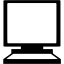
\includegraphics[width=1em]{computer.png}}
\newcommand{\IconCalc}{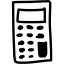
\includegraphics[width=1em]{calculator.png}}
\newcommand{\IconThink}{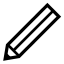
\includegraphics[width=1em]{pencil.png}}
\newcommand{\IconCheck}{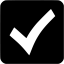
\includegraphics[width=1em]{checkmark.png}}
\newcommand{\IconConcept}{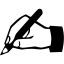
\includegraphics[width=1em]{edit.png}}

\newlength{\SmileysLength}
\setlength{\SmileysLength}{\labelwidth}\addtolength{\SmileysLength}{\labelsep}

\newcommand{\calc}{\hspace*{-\SmileysLength}\makebox[0pt][r]{\IconCalc}%
   \hspace*{\SmileysLength}}
\newcommand{\software}{\hspace*{-\SmileysLength}\makebox[0pt][r]{\IconPc}%
   \hspace*{\SmileysLength}}
\newcommand{\teoria}{\hspace*{-\SmileysLength}\makebox[0pt][r]{\IconThink}%
   \hspace*{\SmileysLength}}
\newcommand{\conceito}{\hspace*{-\SmileysLength}\makebox[0pt][r]{\IconCheck}%
   \hspace*{\SmileysLength}}
\newcommand{\concept}{\hspace*{-\SmileysLength}\makebox[0pt][r]{\IconCheck}%
   \hspace*{\SmileysLength}}

\newcommand*\tipo{Lista de Exercícios - Mínimos Quadrados}
%\newcommand*\turma{...}
\newcommand*\disciplina{ANN0001/CAN0001}
\newcommand*\eu{Helder G. G. de Lima}
\newcommand*\data{\today}

\author{\eu}
\title{\tipo}
\date{\data}

\begin{document}

\begin{center}

\includegraphics[width=9.0cm]{marca} \\
\textbf{\tipo} \\
Prof. \eu\footnote{
Este é um material de acesso livre distribuído sob os termos da licença \href{https://creativecommons.org/licenses/by-sa/4.0/deed.pt_BR}{Creative Commons BY-SA 4.0}.}
\end{center}

%\section*{Legenda}
%\begin{multicols}{4}
%\begin{itemize}
%\item[] \hspace*{\SmileysLength} \calc \hspace*{-\SmileysLength} Cálculos
%\item[] \hspace*{\SmileysLength} \conceito \hspace*{-\SmileysLength} Conceitos
%\item[] \hspace*{\SmileysLength} \teoria \hspace*{-\SmileysLength} Teoria
%\item[] \hspace*{\SmileysLength} \software \hspace*{-\SmileysLength} Software
%\end{itemize}
%\end{multicols}

\section*{Questões}

\begin{enumerate}
\item Obtenha a reta que melhor se ajusta (por mínimos quadrados) aos pontos
$A = (-3, -5)$,
$B = (-2,  7)$,
$C = (-1,  0)$,
$D = ( 0,  1)$,
$E = ( 1,  2)$,
$F = ( 2,  1)$,
$G = ( 3,  2)$,
$H = ( 4,  1)$.
\item Utilize a regressão por mínimos quadrados para ajustar (a) uma reta, (b) uma parábola e (c) uma função da forma $f(x) = k_1 + k_2 \cos(\pi x) + k_3 x^2$ aos seguintes dados, e determine em qual dos três casos o erro quadrático é menor:
\begin{center}
\begin{tabular}{|c|c|c|c|c|c|c|c|}
\hline
   $x_i$ & -3 & -2 & -1 &  0 & 1 & 2 & 3 \\ \hline
$y_i$ & 14 &  4 &  4 & -2 & 2 & 0 & 8 \\
\hline
\end{tabular}
\end{center}

\item Considere um conjunto de pontos $D = \{(x_1,y_1), \ldots, (x_n,y_n)\}$. Classifique as afirmações a seguir como verdadeiras ou falsas, justificando suas respostas:
\begin{enumerate}
\item A função afim que melhor se ajusta a $D$ nunca tem o mesmo erro/resíduo quadrático que o polinômio de grau no máximo dois que melhor se ajusta a $D$.
\item O resíduo quadrático de uma função $f(x) = a_1 + a_2 x$ que melhor se ajusta a $D$ sempre é maior ou igual ao de uma função $g(x) = a_1 + a_2 x + a_3 x^2$ que melhor se ajusta a $D$.
\item O resíduo quadrático da reta que melhor se ajusta a $n$ pontos é maior ou igual ao da reta que se ajusta a $n-1$ destes mesmos pontos.
\end{enumerate}

\item Obtenha a função racional do tipo $f(x) = \frac{a}{x} + \frac{b}{x^2}$ que melhor se ajusta aos pontos do conjunto $D = \{ (1, 3), (2, 0), (2, -2), (5, -1) \}$, no sentido dos mínimos quadrados.

\item Seja $D = \{ (-1,2), (0,3), (1, k) \}$. Determine os valores de $k \in \R$ para os quais o erro quadrático da reta que melhor se ajusta a $D$ é menor do que $2/3$.

\item Encontre as funções afins que melhor se ajustam, no sentido dos mínimos quadrados a:
\begin{multicols}{2}
\begin{enumerate}
   \item $f(x) = e^x$ no intervalo $[-1, 1]$.
   \item $f(x) = \cos(x)$ no intervalo $[0, \pi]$.
\end{enumerate}
\end{multicols}
\end{enumerate}


\newpage
\section*{Algumas respostas}

\begin{enumerate}
\item $f(x) = x/4 + 1$
\item \begin{enumerate}
\item $f(x) = -x + \frac{30}{7} \approx -x + 4.2857142857$, com resíduo quadrático $R \approx 143,43$.
\item $f(x) = \frac{25}{21}x^2 - x-\frac{10}{21} \approx 1.1904761905x^2 - x - 0.4761904762$, com resíduo quadrático $R \approx 24,38$.
\item $f(x) = x^2 - 2\cos(\pi x)$, com resíduo quadrático $R = 28$.
\end{enumerate}
A segunda função apresenta o menor erro quadrático.
\item
\begin{enumerate}
\item \textbf{Falso}. Por exemplo, se $D = \{(1,5), (2,5), (3,5)\}$, então a função constante $y = 5$ é a função que melhor se ajusta aos dados, tanto no caso de funções afins quanto no caso das funções de grau menor ou igual a dois, e seu resíduo é nulo.
\item \textbf{Verdadeiro}. Toda função $f(x) = a_1 + a_2 x$ também pode ser escrita na forma $f(x) = a_1 + a_2 x + 0 x^2$, ou seja, a função $g$ que melhor se ajusta a $D$ não pode ser pior do que $f$, isto é, deve ter um erro quadrático menor ou igual ao de $f$.
\item \textbf{Verdadeiro}. De fato,
\begin{align*}
R(n\ \text{pontos})
& = \sum_{i=1}^n (f(x_i)-y_i)^2
= (f(x_n)-y_n)^2 + \sum_{i=1}^{n-1} (f(x_i)-y_i)^2 \\
& \geq \sum_{i=1}^{n-1} (f(x_i)-y_i)^2
= R(n-1\ \text{pontos}),
\end{align*}
pois $(f(x_n)-y_n)^2 \geq 0$.
\end{enumerate}
\item $f(x) = \frac{-7}{x} + \frac{10}{x^2}$
\item $2 < k < 6$

\item \begin{enumerate}
   \item Se $y = a x + b$ é a função afim procurada, então $X = (a, b)^T$ é solução de $A X = B$, em que

   \[
      a_{11} = \int_{-1}^1 x^2 \diff{x} = \frac{2}{3}
   \]
   \[
      a_{12} = a_{21} = \int_{-1}^1 x \diff{x} = 0
   \]
   \[
      a_{22} = \int_{-1}^1 1 \diff{x} = 2
   \]
   \[
      b_1 = \int_{-1}^1 xe^x \diff{x} = \frac{2}{e}
   \]
   \[
      b_2 = \int_{-1}^1 e^x = e - \frac{1}{e}
   \]
   Assim,
   \[
      \begin{bmatrix}
         \frac{2}{3} & 0 \\
         0 & 2
      \end{bmatrix}
      \cdot
      \begin{bmatrix}
         a \\
         b
      \end{bmatrix}
      =
      \begin{bmatrix}
         \frac{2}{e} \\
         e - \frac{1}{e}
      \end{bmatrix}.
   \]
   Logo, $a = \frac{\frac{2}{e}}{\frac{2}{3}} = \frac{3}{e}$, $b = \frac{e - \frac{1}{e}}{2} = \frac{e}{2} - \frac{1}{2e}$ e assim, $y = \frac{3}{e} x + \frac{e}{2} - \frac{1}{2e}$.


   \item Se $y = a x + b$ é a função afim procurada, então $X = (a, b)^T$ é solução de $A X = B$, em que

   \[
      a_{11} = \int_0^\pi x^2 \diff{x} = \frac{\pi^3}{3}
   \]
   \[
      a_{12} = a_{21} = \int_0^\pi x \diff{x} = \frac{\pi^2}{2}
   \]
   \[
      a_{22} = \int_0^\pi 1 \diff{x} = \pi
   \]
   \[
      b_1 = \int_0^\pi x\cos(x) \diff{x} = -2
   \]
   \[
      b_2 = \int_0^\pi \cos(x) = 0
   \]
   Assim,
   \[
      \begin{bmatrix}
         \frac{\pi^3}{3} & \frac{\pi^2}{2} \\
         \frac{\pi^2}{2} & \pi
      \end{bmatrix}
      \cdot
      \begin{bmatrix}
         a \\
         b
      \end{bmatrix}
      =
      \begin{bmatrix}
         -2 \\
         0
      \end{bmatrix}.
   \]
   Por Cramer, como $\begin{vmatrix}
      \frac{\pi^3}{3} & \frac{\pi^2}{2} \\
      \frac{\pi^2}{2} & \pi
   \end{vmatrix} = \frac{\pi^4}{3} - \frac{\pi^4}{4} = \frac{\pi^4}{12}$, tem-se $a = \frac{\begin{vmatrix}
      -2 & \frac{\pi^2}{2} \\
      0 & \pi
   \end{vmatrix}}{\frac{\pi^4}{12}} = \frac{-2\pi}{\frac{\pi^4}{12}} = -\frac{24}{\pi^3}$ e  $b = \frac{\begin{vmatrix}
      \frac{\pi^3}{3} & -2 \\
      \frac{\pi^2}{2} & 0
   \end{vmatrix}}{\frac{\pi^4}{12}} = \frac{\pi^2}{\frac{\pi^4}{12}} = \frac{12}{\pi^2}$. Assim, $y = -\frac{24}{\pi^3} x + \frac{12}{\pi^2}$.
\end{enumerate}
\end{enumerate}
\end{document}
